%!TEX root = ../../main.tex


\begin{figure}[!htb]
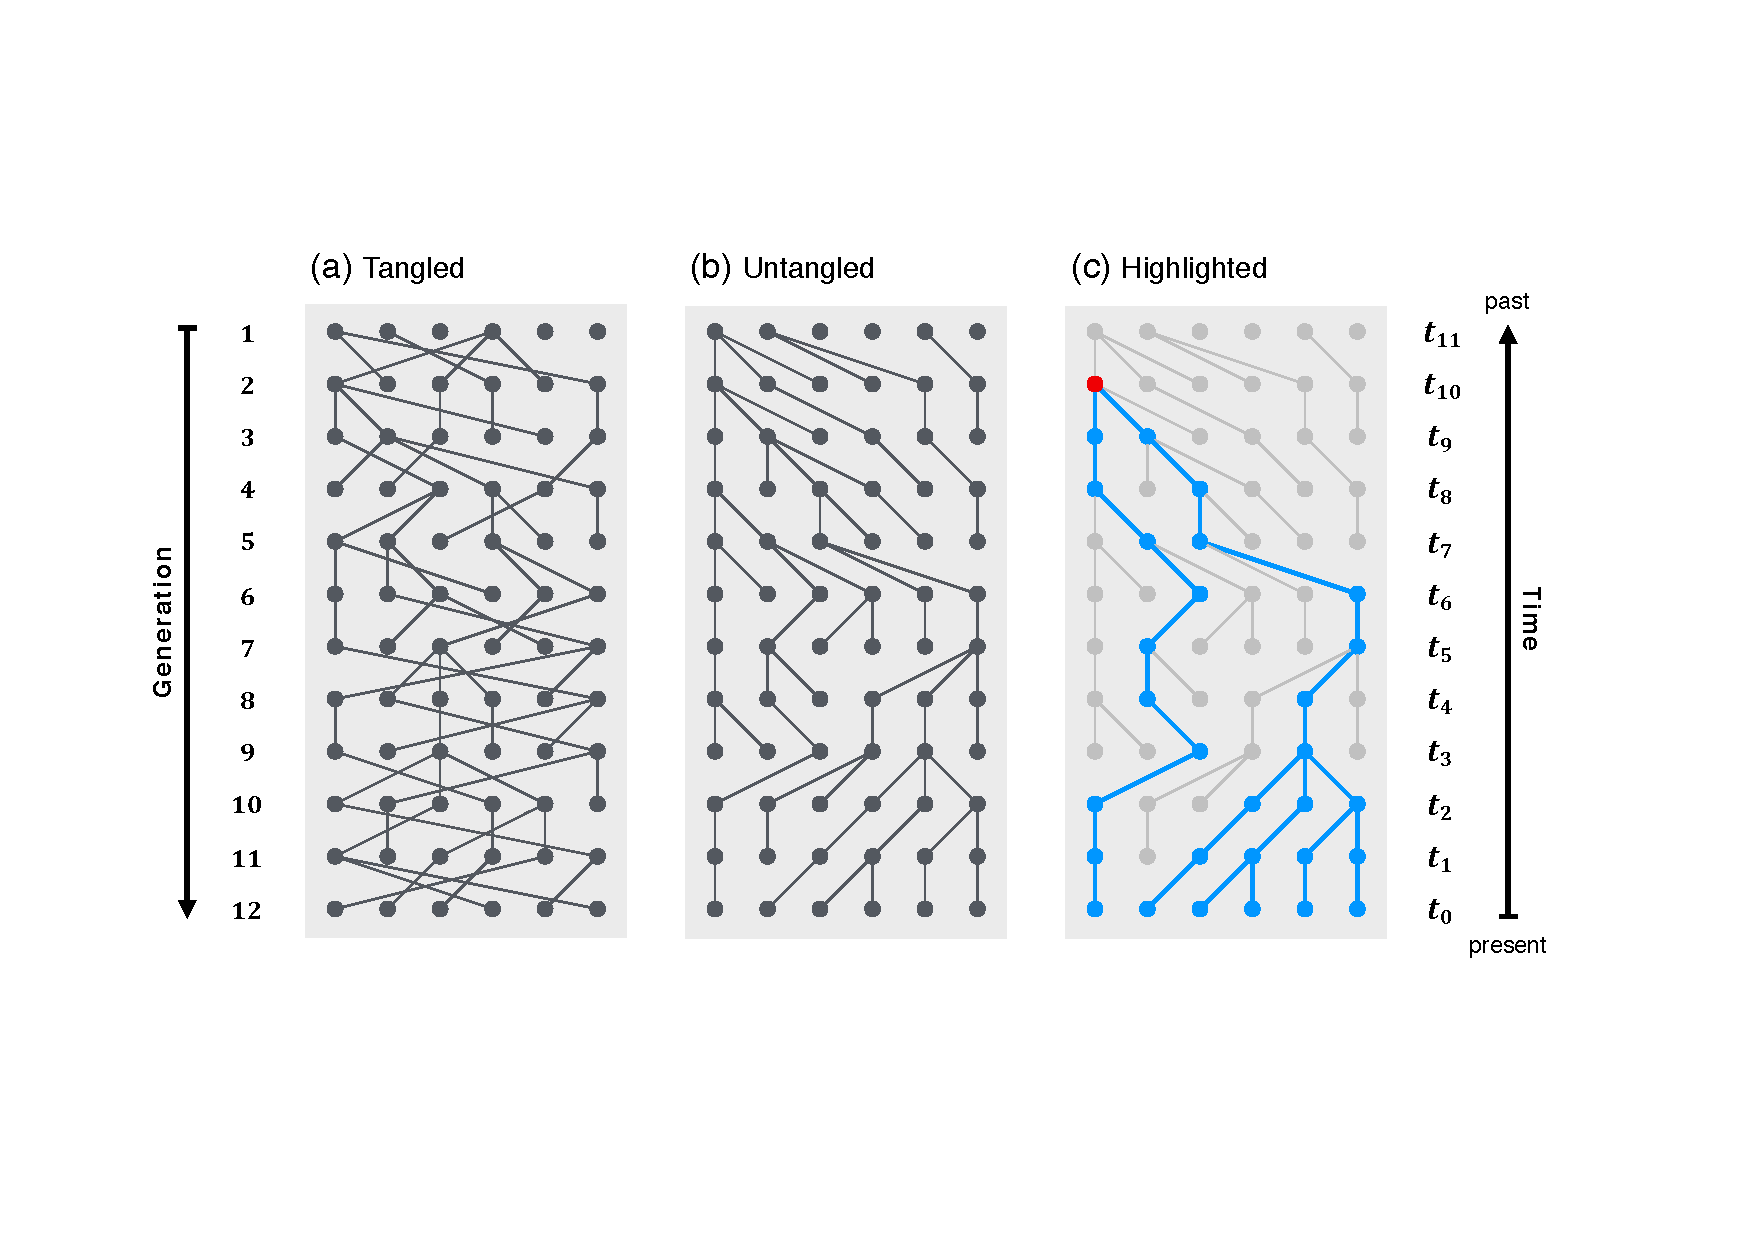
\includegraphics[width=\textwidth]{./img/ch1/info_wrightfisher}
\Caption{Example genealogy in a Wright-Fisher model}
{A population of size ${N=6}$ is shown in Panel~\textbf{(a)}, which is observed over 12 generations.
In the neutral Wright–Fisher model, \n{1} individual is chosen at random (with replacement) in each generation to produce offspring for the next generation, repeated $N$~times.
The genealogy of the population is more clearly seen after individuals have been sorted such that their lineages do not cross; see Panel~\textbf{(b)}.
Note that not every individual produces offspring, such that some lineages go extinct.
If this process is repeated over many generations (forward in time), it can be seen that all individuals in the present generation derive from a single individual in the past, which is indicated in Panel~\textbf{(c)}.
The ancestry of the present population (\emph{blue}) is traced back to a single ancestor (\emph{red}) at time ${t=10}$~generations ago.}
{fig:info_wrightfisher}
\end{figure}
